\section{溶液作製精度による影響}

溶液の作製精度の確認を行うため,0.95,1.00,1.05wt.\%のPAA溶液を作製した.それぞれの擬塑性流体に直径10mmの鋼球を落下させ,終端速度の変化,超音波照射による影響の変化の確認を行った.

\subsection{溶液の粘性特性に関して}
それぞれの溶液の特性を確認するため,粘度計を用いて粘度計測を行った.粘度計測を行った結果をFig.\ref{fig:95-105}に示す.比較のため,先行研究である岩室\cite{ref:8}とShiratori \textit{et al}.\cite{ref:9}の計測結果も合わせて示す.また,Power-law modelに従うものとして,式(\ref{eq:power-low})を用いて近似計算を行った結果をTable\ref{table:005_knParameter}に示す.濃度が薄いと粘度は低く,濃度が高いと粘度は高くなった.

\begin{figure}[H]
    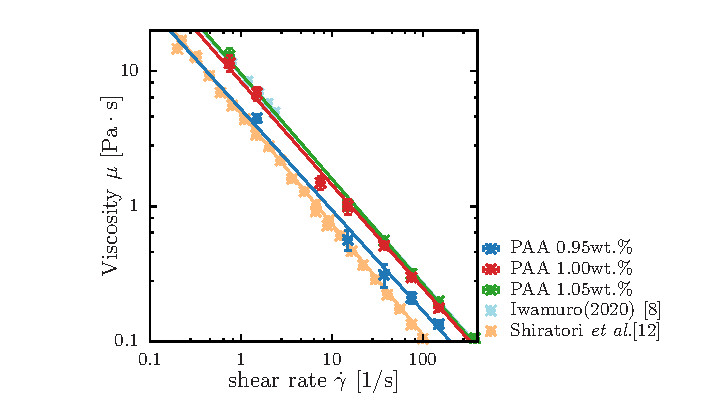
\includegraphics[width=0.72\textwidth]{X-Appendix/concentration/viscosity/viscosity.eps}
    \caption{Viscosity versus shear rate for PAA0.95,1.00,1.05wt.\%.}
    \label{fig:95-105}
\end{figure}

\begin{table}[H]
    \centering
    \caption{Parameters $k$ and $n$ in the Power-law model for each PAA solution.}
    \label{table:005_knParameter}
    \begin{tabular}{c|c|c} \hline
                                                     & $k$ & $n$  \\ \hline \hline
        Present Value(1.05wt.\%)                     & 9.6 & 0.23 \\
        Present Value(1.00wt.\%)                     & 8.4 & 0.24 \\
        Present Value(0.95wt.\%)                     & 5.2 & 0.25 \\
        岩室\cite{ref:8}                             & 9.4 & 0.23 \\
        Shiratori \textit{et al}.(2016)\cite{ref:10} & 5.9 & 0.25 \\ \hline
    \end{tabular}
\end{table}

\subsection{溶液の作製精度による高速化への影響}

ぞれぞれの質量濃度のPAA溶液に対し,落下球実験を行った.落下させた球は,鋼製の直径10mmの球である.実験結果をFig.\ref{fig:95-105velocity}に示す.この結果より,超音波照射されていない状態における落下球の終端速度をFig.\ref{fig:95-105_cal}(a)に示す.溶液濃度変化によって大きな終端速度の変化は見られなかったが,溶液濃度が濃い場合,わずかに終端速度が遅かった.これは,粘性が強いためであると考えられる.溶液濃度と超音波照射による高速化度合の関係をFig.\ref{fig:95-105_cal}(b)に示す.濃度が濃くなるとより高速化が顕著になった.これは,溶液粘度が高くなり,より強い擬組成を示したためであると考えられる.超音波照射による高速化度合を粘度比と音響境界層を球の半径で規格化した値の関係をFig.\ref{fig:95-105_cal}(c)に示す.他の実験によって得られた結果も示す.本研究の粘度比の範囲と比較して,今回行った実験範囲は非常に狭い範囲であることが分かる.また,今回の濃度変化による粘度比と高速化度合の関係は他の実験結果と同様の正の相関関係が見られた.

以上より,$\pm$0.05wt.\%の濃度変化をさせた場合,粘度,終端速度,高速化度合,粘度比にわずかながら変化を示すことが分かった.粘度比と高速化度合の関係は他の結果と同様の結果が得られることが分かった.これらの結果より,実験の都度,粘度計測を行い,球を落下させた時のせん断粘度特性を得ることが重要であることが分かった.

\begin{figure}[H]
    \centering
    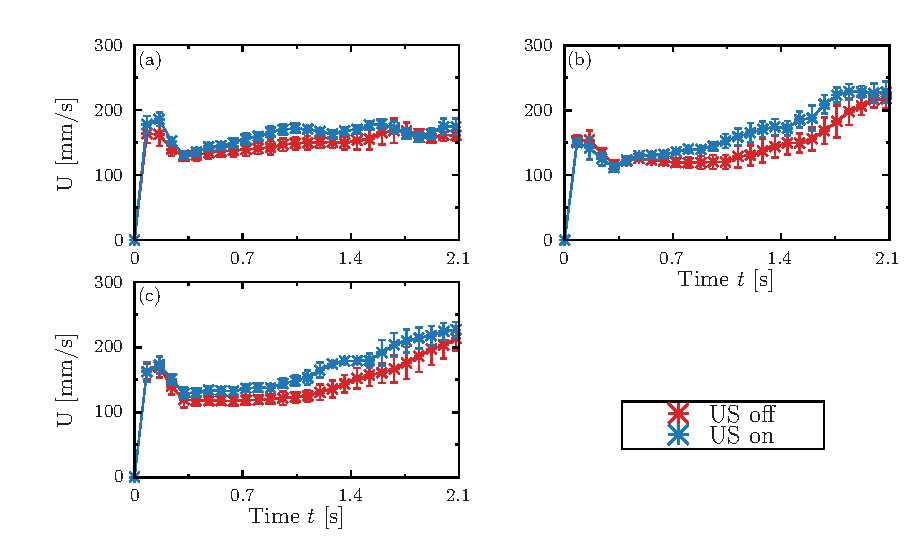
\includegraphics[width=0.9\textwidth]{X-Appendix/concentration_diff/concentration_diff.eps}
    \caption{Velocity of a falling sphere in (a)0.95wt.\%, (b)1.00wt.\%, (c)1.05wt.\% PAA solution.}
    \label{fig:95-105velocity}
\end{figure}

\begin{figure}[H]
    \centering
    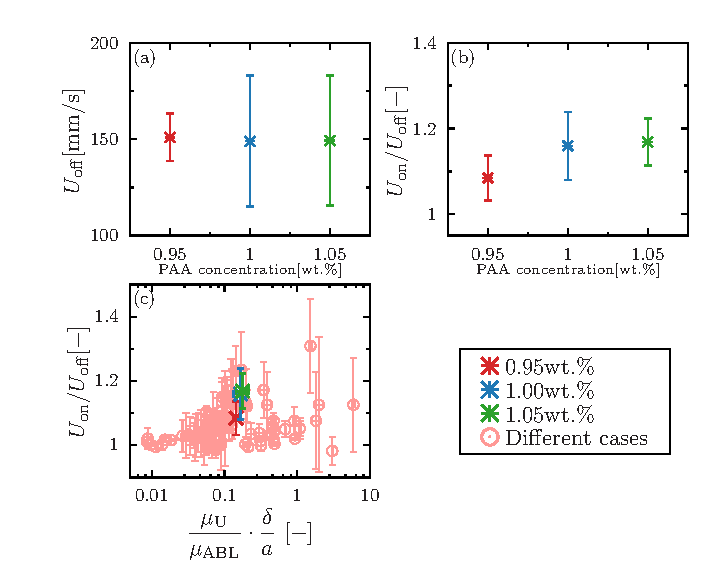
\includegraphics[width=1\textwidth]{X-Appendix/concentration_diff/concentration_diff_cal.eps}
    \caption{Relationship between (a)terminal velocity and PAA concentration, velocity ratio and (b) PAA concentration, (c)viscosity ratio.}
    \label{fig:95-105_cal}
\end{figure}
